\documentclass[a4paper, 10pt]{article}
\usepackage[english]{babel}
\usepackage[utf8]{inputenc}
\usepackage{amsfonts}
\usepackage{graphicx}
\usepackage{placeins}
\usepackage[hidelinks]{hyperref}

\author{Maarten de Jonge}
\title{Projective Geometric Algebra}

\begin{document}
\newcommand{\rp}{$\mathbb{R}^{3,3}$ }

\maketitle

\section{Introduction}
This introduction gives a short overview of various concepts essential to
this thesis, mainly projective geometry and geometric algebra. Subsequently,
these are tied together and the topic of this research emerges.

\subsection{Projective Geometry}
Projective geometry is the study of geometric properties invariant under
projective transformations, with applications in areas such as computer vision,
computer graphics, and quantum physics. Compared to the familiar Euclidean
geometry, the space is extended with elements at infinity. This solves a number
of irregularities and adds a greater expressive power to the algebra. For
example, two different lines in the same plane in Euclidean geometry have either
one or zero (when the lines are parallel) points of intersection. With the
addition of points at infinity, this becomes more general: two different lines
in the same plane always have one point of intersection, where parallel lines
will meet in infinity. This mimics observations in real life, e.g. train tracks
which appear to converge as the distance increases, eventually
appearing to meet at an infinite distance even though they are obviously parallel.
An important advantage of this is in software implementation: you will not have
to check for edge cases when there are no edge cases, leading to both simpler
and more efficient implementations.

\subsection{Geometric Algebra}
Geometric algebra\cite{dorst2009geometric} is an algebra over an $n$-dimensional
vector space, similar to
linear algebra. Unlike linear algebra however, geometric algebra allows for
coordinate-free transformations in a structure-preserving manner by using the
geometric product. Of further note is the outer product, which constructs
higher-dimensional subspaces from basic elements. Of the various models of
geometric algebra in use, the homogenous model is of most interest for this thesis.
This model embeds $n$-dimensional space in an $n + 1$-dimensional representational
space (similarly to the homogenous model of linear algebra).  Lines are
represented as the outer product of two vectors (which themselves represent
points); this is referred to as a \emph{2-blade} or more generally a
\emph{bivector}. These line elements can be represented as vectors on a basis of
$n \choose 2$ bivectors (the amount of unique bivectors in $n$-dimensional
space), leading to a space which uses lines as its basis elements (a \emph{line
space}). Applying this to lines in homogeneous 3D space leads to an equivalence
with Pl\"{u}cker coordinates, a system for representing 3D lines by means of 6
homogeneous coordinates. This results in a system referred to as the Pl\"{u}cker
model of geometric algebra.

\subsection{Research Topic}
Recent research of the Pl\"{u}cker model (done by \cite{hangbo2011}
\cite{dorst2013versors} \cite{pottmann2001computational} \cite{dekok2012} as
elaborated on in section 2) has provided the geometric elements of the space
with visual interpretations. GAViewer, a geometric algebra visualisation tool
which currently has partial support for the Pl\"{u}cker model, will be extended
with a particularly tricky 3-blade whose visualisation is in the form of a
regulus (figure \ref{fig:regulus}).

In addition, the Pl\"{u}cker model will be applied to 2D projective geometry by
taking a cross-section of a regulus to be a conic section in 2D and considering
only transformations which keep this cross-section constant. The focus will lie
on the following projective geometrical concepts:
\begin{itemize}
  \item Testing for membership of a point to a conic section.
  \item The duality between a point and a line relative to a conic section.
\end{itemize}

\begin{figure}[htbp]
  \centering
  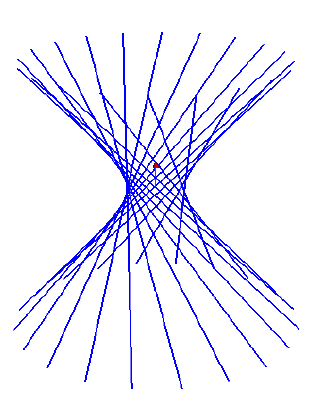
\includegraphics[width=0.5\textwidth]{regulus.png}
  \caption{A regulus}
  \label{fig:regulus}
\end{figure}

\bibliographystyle{plain}
\bibliography{library}
\end{document}
